% !TeX encoding = UTF-8
% !TeX spellcheck = de_DE

%% Dies gibt Warnungen aus, sollten veraltete LaTeX-Befehle verwendet werden
\RequirePackage[l2tabu, orthodox]{nag}

\documentclass[utf8,biblatex]{lni}
\bibliography{lni-paper-example-de}

%% Schöne Tabellen mittels \toprule, \midrule, \bottomrule
\usepackage{booktabs}
\usepackage[ngerman]{babel}
%% Zu Demonstrationszwecken
\usepackage[math]{blindtext}
\usepackage{mwe}

%% BibLaTeX-Sonderkonfiguration,
%% falls man schnell eine existierende Bibliographie wiederverwenden will, aber nicht die .bib-Datei händisch anpassen möchte.
%% Bitte \iffalse und \fi entfernen, dann ist diese Konfiguration aktiviert.

\iffalse
\AtEveryBibitem{%
  \ifentrytype{article}{%
  }{%
    \clearfield{doi}%
    \clearfield{issn}%
    \clearfield{url}%
    \clearfield{urldate}%
  }%
  \ifentrytype{inproceedings}{%
  }{%
    \clearfield{doi}%
    \clearfield{issn}%
    \clearfield{url}%
    \clearfield{urldate}%
  }%
}
\fi

\begin{document}

%%% Mehrere Autoren werden durch \and voneinander getrennt.
%%% Die Fußnote enthält die Adresse sowie eine E-Mail-Adresse.
%%% Das optionale Argument (sofern angegeben) wird für die Kopfzeile verwendet.
\title[Software Reuse]{Software Reuse: Überblick und Anwendung}
%%%\subtitle{Untertitel / Subtitle} % falls benötigt
\author[Adrian Liehner \and Jülf Freudenberger]
{Adrian Liehner\footnote{DHBW Stuttgart Campus Horb, Informatik, Florianstraße 15, 72160 Horb am Neckar, Deutschland \email{i20023@hb.dhbw-stuttgart.de}} \and
 Jülf Freudenberger\footnote{DHBW Stuttgart Campus Horb, Informatik, Florianstraße 15, 72160 Horb am Neckar, Deutschland \email{i20013@hb.dhbw-stuttgart.de}}}
%\startpage{11} % Beginn der Seitenzählung für diesen Beitrag
%\editor{Herausgeber et al.}    % Namen der Herausgeber
\booktitle{Software Engineering II} % Name des Tagungsband; optional Kurztitel
\yearofpublication{2022}
%%%\lnidoi{18.18420/provided-by-editor-02} % Falls bekannt
\maketitle


\begin{abstract}
Methoden und Werkzeuge, welche in der Entwicklung von Software Anwendung finden, unterliegen einem stetigen Wandel. Stets denken Entwickler darüber nach, wie sich der Prozess der Softwareentwicklung noch effizienter gestalten lässt. Ein in diesem Kontext häufig genannter Begriff ist \textbf{Software Reuse}. 

Diese Arbeit zeigt auf, was Software Reuse ausmacht, welche Aspekte bei der Softwareentwicklung Wiederverwendet werden können und worauf bei der Wiederverwendung von Software zu achten ist. Es wird auf Software Reuse und Code Reuse eingegangen und erläutert, wie Software Reuse mit der Qualität der Software zusammen hängt. Außerdem wird auf Metriken eingegangen, die bei Software Reuse relevant sind. Des Weiteren werden einige Software Architekturmuster erläutert und deren Stärken und Schwächen bezüglich Software Reuse aufgezeigt.
\end{abstract}

\section{Was ist Software Reuse?}

Bei Softwaere Reuse geht es um die Entwicklung von Software unter der Verwendung bereits bestehender Software-Komponenten. Als Komponenten können hier sowohl Quellcode, wie auch Software-Design, Schnittstellen, Anleitungen, Dokumentation oder auch Anforderungsspezifikationen verstanden werden \cite{T4Tutorials.com.04.11.2022}. 

Software Reuse wird auch als Code Reuse oder als wiederverwendungsorientiertes Software Engineering bezeichnet.

Bei der Entwicklung von Software suchen Unternehmen Möglichkeiten, den Entwicklungsprozess zu beschleunigen und Kosten zu sparen. Deshalb ist es wichtig zu verstehen, worum es bei Software Reuse geht und wie Wiederverwendung von Software erfolgreich durchgeführt werden kann.

\textbf{Historischer Kontext}

Die Idee von der Wiederverwendung von Programmcode gibt es schon seit es Computer gibt, so beschrieb bereits Charles Babbage, wie eine Bibliothek an Lochkarten seiner \glqq Analytical Engine \grqq \space Programme enthalten könnten, die wiederverwendet werden. 
\cite{Wikipedia.2022}

Allerdings geht es bei Software Reuse weniger um die Wiederverwendung von Programmen selbst, sondern mehr um die Wiederverwendung verschiedener Elemente der Softwareentwicklung wie Quellcode beim erstellen einer neuen Software.  

Was heute unter Software Reuse verstanden wird, wurde erstmals von McIlroy \cite{NATO.1968} im Jahr 1968 in seinem Paper "Mass produced software components" beschrieben, welches er auf der NATO Software Engineering Conference im Jahr 1968 veröffentlichte. Darin beschreibt er die Idee von massenproduzierten Softwarekomponenten und zieht Vergleiche zu der Standardisierung von Schrauben und elektronischen Widerständen. Er zeigt auf, dass beim Erstellungsprozess neuer Software meist die Frage \glqq Welche Mechanismen sollen wir bauen?\grqq \space statt \glqq Welche Mechanismen sollen wir verwenden?\grqq \space zur Diskussion steht. McIlroy ist der Meinung, dass es an der Zeit ist, Software wiederzuverwenden. \cite{NATO.1968}

Mit seiner Aussage hat McIlroy völlig recht, da er im Gegensatz zu früheren Ideen der Wiederverwendung von Software durch die Technologie seiner Zeit verschiedene Möglichkeiten hat, Software öfters zu verwenden. So bot beispielsweise die in den 60-er Jahren entwickelte Objektorientierte Programmiersprache Simula \cite{Nygaard.1982} die Möglichkeit, Klassen in Bibliotheksdateien auszulagern und diese zum Zeitpunkt der Kompilierung zu verwenden. 

Die Gedanken von McIlroy, Software wiederzuverwenden, werden im Laufe der Jahre in verschiedenen Formen in die Softwareentwicklung Einzug erhalten. Dazu tragen beispielsweise eine Vielzahl an Programmiersprachen bei, welche konzeptionell auf die Mehrfachverwendung von Quellcode ausgelegt sind - zum Beispiel wie bereits erwähnt über Objektorientierte Klassen oder Auslagerung in Bibliotheksdateien. 


\textbf{Einfluss des Internets auf Software Reuse}


Die Erfindung des Internets hatte auf die Menschheit einen unberechenbaren Einfluss. Sehr viele Dinge, die zuvor nur offline möglich waren, konnten nun im Internet erledigt werden, wie Einkaufen, mit anderen Menschen kommunizieren oder das Lesen von Nachrichten oder Büchern. 

In den Anfängen der Softwareentwicklung war so ziemlich jede Software in den USA öffentlich zugänglich, da Software meist hoch spezialisiert und dadurch von geringem Wert war. Erst im Laufe der Zeit entwickelte sich eine Softwareindustrie, der es um den kommerziellen Verkauf von Softwareprodukten ging.

Es war gang und gebe, dass Nutzer Software verbessern oder Fehler selbst beheben und diese selbstständig anderen über IBMs SHARE oder DECTUS zur Verfügung stellten. Software wurde physikalisch auf Magnetband, Floppy Discs oder Compact Discs ausgeliefert und transportiert. 

Die heutigen Softwareprodukte unterschieden sich stark von den aus den 80er und 90er Jahren. Das Internet ermöglichte den Softwareunternehmen, ihre Produkte elektronisch auszuliefern. 

Neue Anwendungstypen und technologische Fortschritte sorgten auch für neue Werkzeuge, die zur Anwendungsentwicklung genutzt werden konnten \cite{Wasserman.2011}. Während Entwicklerteams zuvor noch gemeinsam an einem Ort arbeiteten ermöglichte das Internet globale Kommunikation, was Remote-Entwicklung möglich machte. So erhielten auch erste Internet-angebundene Projekte Repositorys, welche Quellcode und Dokumentation beinhalteten, Einzug in die Softwareentwicklung. Die ersten Repository-Plattformen SourceForge, Google Code und GitHub begannen hunderttausende Open Source Projekte zu hosten. Durch diese Entwicklung wurde die Wiederverwendung von Software so Mainstream wie sie heute ist.


Gerade durch Werkzeuge wie GitHub \cite{GitHub.04.11.2022} und Stack Overflow \cite{StackOverflow.04.11.2022} hat sich der Prozess der Softwareentwicklung in den letzten Jahren stark verändert. Viele Funktionalitäten die Entwickler zuvor selbst programmieren mussten, können heute einfach aus dem Internet übernommen werden. Die meisten Probleme, die beim Programmieren auftreten, hatte jemand anders bereits erlebt und es ist möglich, dass eine einfache Google-Suche ein schnelles Ergebnis liefert. 

Ein ausformuliertes Konzept, wie Softwareentwickler im Internet nach Quellcode suchen, haben viele Unternehmen nicht, es ist meist dem Entwickler selbst überlassen, wie er mit dem Werkzeug, welches ihm zur Verfügung steht umgeht, und wie er Onlineressourcen in seine Entwicklung einfließen lässt. Ein Grund dafür ist, dass Entwickler unterschiedliche Kenntnissstände haben. Ist einem Entwickler die Lösung für ein spezifisches Problem möglicherweise bereits auf früheren Entwicklungen bekannt, so wird er es mit der ihm bekannten Methode lösen. Weniger erfahrene Entwickler greifen hingegen schneller zu Online-Ressourcen um ihre Probleme zu lösen. 

Aktuelle Entwicklungen im Bereich der Künstlichen Intelligenz lassen vermuten, wie Softwareentwicklung in Zukunft aussehen könnte. KI-Werkzeuge, wie das auf OpenAI´s GPT-3 basierte GitHub Copilot, können Softwareentwickler bei ihrer Arbeit unterstützen. Das Neuronale Netzwerk durchsucht Milliarden Zeilen an Code, um dem Entwickler eine Lösung für sein Problem zu präsentieren. Diese moderne Form von KI-basierter Softwareentwicklung könnte die automatisierte Zukunft von Software Reuse darstellen. 



\section{Arten von Software Reuse}


Wenn wir von Software Reuse sprechen, ist es erforderlich zwischen der Wiederverwendung von Quellcode und der Entwicklung von wiederverwendbarem Quellcode unterscheiden. 

Bei der Wiederverwendung von Quellcode muss der Entwickler nach \citet{Bauer.2016} zunächst herausfinden, für welche Funktionalität er Quellcode wiederverwenden möchte. Er muss evaluieren ob es sich überhaupt lohnt für sein Problem Quellcode wiederzuverwenden, oder ob der Aufwand zu groß ist und er den Code selbst schreiben sollte. Anschließend muss er Programmcode finden, der sich für sein Problem anwenden lässt. Umso genauer der verwendete Code für das Projekt passt, umso weniger Aufwand hat der Entwickler bei der Anpassung und Implementation des Quellcodes in sein Projekt. 

Ganz anders muss ein Entwickler vorgehen, der Quellcode entwickeln möchte, welcher möglichst wiederverwendbar sein soll. Er muss abwägen, wie viel Zeit und Mehraufwand er investieren kann, um seinen Quellcode wiederverwendbarer zu gestalten. Dabei kann er sich daran orientieren, wie oft sein Quellcode an anderen Stellen oder in anderen Projekten wiederverwendet werden kann, wie viel Wartungsaufwand der Software durch seine Verbesserungen gespart werden kann, die Anzahl der Personen, die von den Verbesserungen profitieren, und die Zeitspanne über die der Quellcode verwendet werden kann \citet{Bauer.2016}. 





\textbf{Art der Artefakte, die wiederverwendet werden}


Software Entwickler haben verschiedene Möglichkeiten Software wiederzuverwenden. In \cite{Bauer.2016} wurden in einer kleinen Umfrage Entwickler eines Entwicklerteams bei Google befragt, wie sie Wiederverwendung durchführen. Die häufigsten Antworten waren:

\begin{figure}[h]
  \centering
  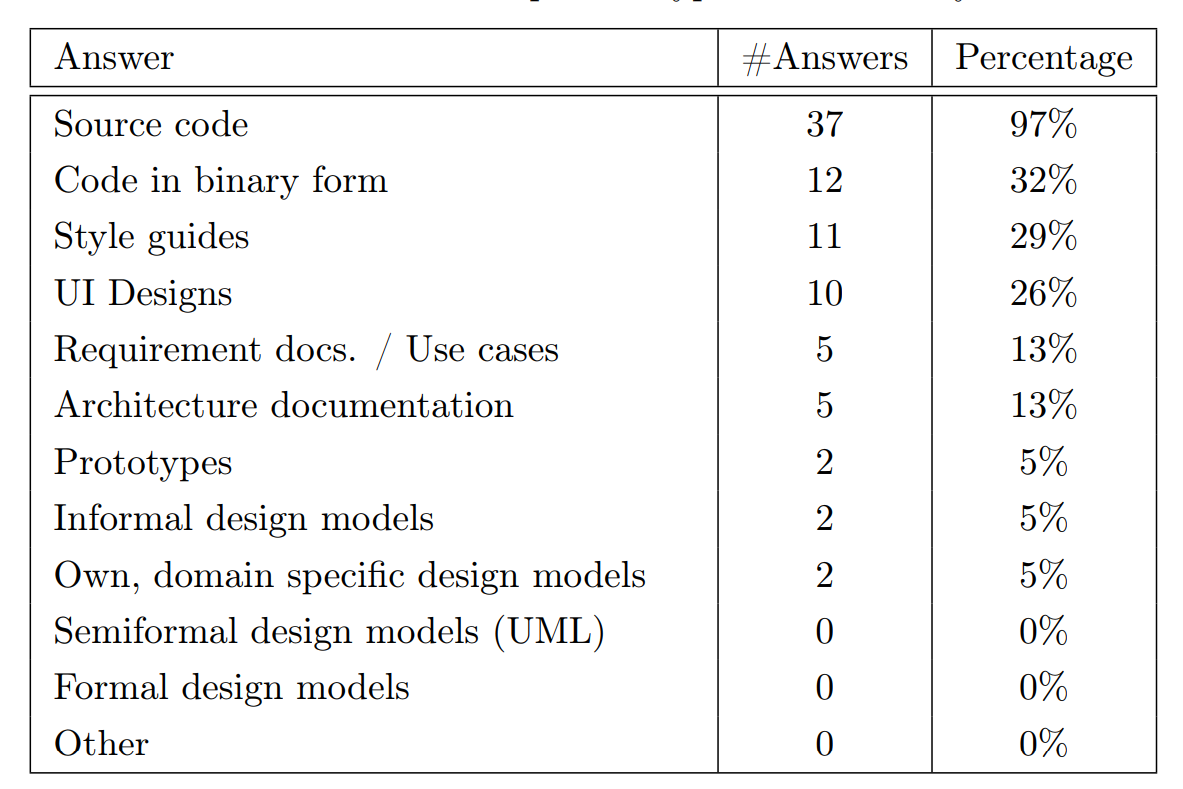
\includegraphics[width=.8\textwidth]{images/image1.png}
  \caption{Wiederverwendung verschiedener Artefakte}
  \label{fig:image1}
\end{figure}

Es ist deutlich zu sehen, das Quellcode am häufigsten wiederverwendet wird, während Design Models eher selten wiederverwendet werden. Das könnte damit zusammenhängen, dass sich die Designspezifikationen zwischen verschiedenen Projekten unterscheiden, sodass eine Wiederverwendung oft nicht sehr sinnvoll erscheint. Es ist allerdings zu beachten, das es sich bei dieser Umfrage nur um eine Stichprobe handelt, und die Grafik nicht repräsentativ für alle Unternehmen ist. 

Wichtig ist also, für das eigene Entwicklerteam eine Analyse durchzuführen, um herauszufinden, in welchem Umfang Software Reuse stattfindet. So kann festgestellt werden, ob potentiell weitere Artefakte der Softwareentwicklung wiederverwendet werden sollten.


Auch gibt es verschiedene Vorgehensweisen, wie Quellcode wiederverwendet werden kann. Auch diese wurden in \cite{WilliamB.FrakesandChristopherJ.Fox.1996} in einer Umfrage ausgewertet. Auch diese Umfrage ist nicht repräsentativ, zeigt allerdings Möglichkeiten zur Wiederverwendung auf. 

\begin{figure}[h]
  \centering
  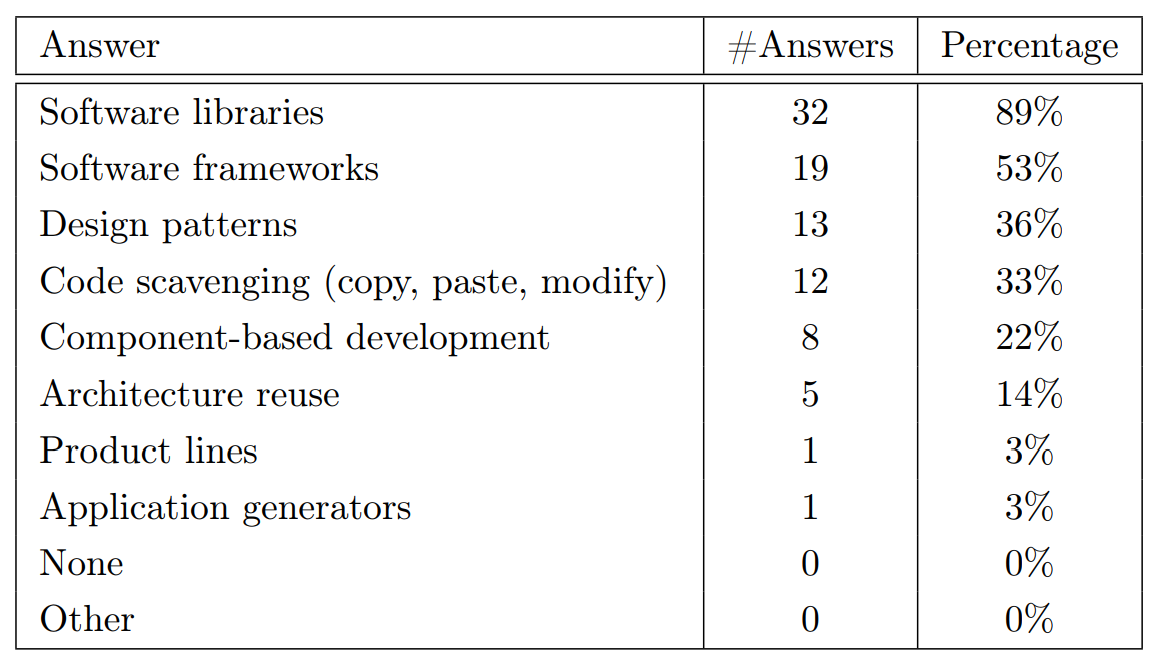
\includegraphics[width=.8\textwidth]{images/image2.png}
  \caption{Wiederverwendung bei der Softwareentwicklung}
  \label{fig:image2}
\end{figure}

Zunächst ist interessant, dass keiner der befragten Entwickler angab, in keiner Weise Wiederverwendung durchzuführen. Das nutzen von Softwarebibliotheken liegt mit großem Abstand vorne, hingegen landet das Kopieren und Einfügen von Quellcode lediglich auf dem vierten Platz.
Als eine grundlegende Erkenntnis lässt sich erkennen, dass das Wiederverwenden von Software in verschiedensten Formen Bestandteil der Vorgehensweise von Entwicklern und aus dem Alltag nicht mehr wegzudenken ist.

Für Entwickler ist es wichtig, selbst zu Analysieren, auf welche Arten Software wiederverwendet wird. So können Potentiale für Software Reuse erkannt werden.  

Die verschiedenen Arten Software wiederzuverwenden sind auch mit unterschiedlich viel Aufwand verknüpft. Während einfaches Kopieren von Code in Sekundenschnelle durchgeführt werden kann, benötigt hingegen die Wiederverwendung einer Softwarearchitektur eine strukturierte Planung und viel Zeit. Je nachdem was wiederverwendet werden soll, müssen unterschiedliche Personen von Entwicklungsteams mit einbezogen werden. Mit steigender Komplexität der Wiederverwendung wächst die Schwierigkeit, die Wiederverwendung erfolgreich und effizient durchzuführen.



\section{Voraussetzungen, Chancen und Risiken von Software Reuse}



\textbf{Vorbereitung für systematische Wiederverwendung}


Nach Frakes and Fox \cite{WilliamB.FrakesandChristopherJ.Fox.1996} gibt es bei der Wiederverwendung von Software verschiedene Aspekte zu beachten, darunter Management und Wirtschaftlichkeit. 

Wenn Software systematisch wiederverwendet werden soll, muss das Management der Organisation, welche die Software entwickelt, Anreize dafür schaffen. Eine Möglichkeit Anreize zu schaffen wäre den monetären Wert aufzuzeigen, welchen eine konkrete Entwicklung eines wiederverwendbaren Softwareteils schafft. 

Indem festgehalten wird, wie oft Software wiederverwendet wird, könnten Organisationen die Entwicklung wiederverwendbarer Softwarekomponenten wirtschaftlich begründen. 


\textbf{Technische Voraussetzungen für erfolgreiche Wiederverwendung von Software}

Damit die Wiederverwendung von Software erfolgreich sein kann, müssen nach \citet{Bauer.2016} bestimmte Rahmenbedingungen gegeben sein. So sollte eine adäquate Infrastruktur vorliegen. Das Projekt an dem gearbeitet wird benötigt eine Art von Quellcodeverwaltung und Versionierung, die es ermöglicht, die einzelnen Entwicklungsschritte nachvollziehen zu können. Außerdem sollte die Software dokumentiert werden, sodass andere Personen, die ebenfalls an der Software arbeiten, leichter verstehen, welche Softwarekomponente wie arbeitet. Bei der Entwicklung sollten die Entwickler auf gute Softwarequalität achten, welche die Lesbarkeit verbessert und Veränderungen am Code, wie zum Beispiel das Refactoring, möglichst unkompliziert zulässt. 



\textbf{Chancen von Software Reuse}


Wiederverwendung von Software findet in Organisationen nur dann statt, wenn daraus Vorteile gezogen werden können. 
Es gibt verschiedene Aspekte welche sich, je nach Strategie und Umsetzung, durch die Wiederverwendung von Software positiv verändern können. So kann die Entwicklungszeit durch Wiederverwendung verkürzt werden, was wiederum die Kosten für die Entwicklung senkt. Je nach Anwendungsszenario können Fehler im Code vermieden werden, indem gut getestete Softwareteile wiederverwendet werden. So kann eine höhere Softwarequalität gewährleistet werden. Bekannte Fehler sind bereits behoben und Softwaretests bereits durchgeführt, wodurch das Endprodukt robuster wird.


\textbf{Risiken von Software Reuse}


Wenn die systematische Wiederverwendung von Software nicht richtig durchgeführt wird, kann diese auch zum Nachteil für die Entwickler und die Organisation werden. 

Aufgezwungene Wiederverwendung von Software kann dazu führen, dass veraltete Technologien zu lange verwendet werden. Dies kann passieren, wenn beispielsweise Aktualisierungen von Frameworks oder Bibliotheken Neuentwicklungen erfordern würden, für welche entweder nicht das Budget oder das Entwickler-Know-how vorhanden ist. Das Potential, welches durch Neuentwicklung mittels aktuellerer Technologien kommt, sollte nicht außer Acht gelassen werden. 

Je nach Anwendungsszenario kann Wiederverwendung von Software auch zu Performanceeinbußen führen. Die Wiederverwendung generischer Komponenten kann zu höherer Speichernutzung führen, wie es eine spezifische Neuentwicklung tun würde. 

Zudem können falsche Praktiken bei der Wiederverwendung von Software dazu führen, das der Code komplizierter zu warten und für neue Entwickler schwerer zu verstehen ist.

\textbf{Reuse Failure Modes Model}


Das Reuse Failure Modes Model wurde in \cite{WilliamB.FrakesandChristopherJ.Fox.1996} erstmals beschrieben und veröffentlicht. Das Modell zeigt verschieden Faktoren auf, die für erfolgreiche Wiederverwendung gegeben sein müssen.

Um zum Erfolg zu gelangen, muss die in \cite{WilliamB.FrakesandChristopherJ.Fox.1996} beschriebene siebenschrittige Reuse Success Chain abgearbeitet werden. Es gibt verschiedene Gründe, weshalb die Wiederverwendung in den einzelnen Schritten fehlschlagen kann.
\begin{enumerate}

    \item \textbf{Es muss ein Versuch stattfinden, Software wiederzuverwenden.}
    
    Es gibt eine Vielzahl an Gründen, weshalb Software Reuse von Punkt eins an nicht stattfindet. 
    Die Wiederverwendung scheitert an diesem Punkte wenn die Ressourcen, welche für die Entwicklung verwendet werden dürfen oder können beschränkt sind, oder an erster Stelle kein Anreiz für die Wiederverwendung gegeben ist. Für die Wiederverwendung muss Zeit zur Verfügung stehen und es muss ein klarer Nutzen aus der Wiederverwendung hervorgehen. Die Entwickler benötigen ausreichende Kenntnisse und Bildung, um die Wiederverwendung durchzuführen. Die Wiederverwendung kann außerdem an unzureichender Kommunikation scheitern. Auch Rechtliche Probleme können zum scheitern der Wiederverwendung führen. Das Management muss die Entwicklung unterstützen und die Organisation der Entwicklung muss die Wiederverwendung ermöglichen. Zudem kann es passieren, das die Kunden des Projektes das wiederverwenden von Software nicht möchten. Zu den selteneren Problemen, weshalb kein Versuch Software wieder zu verwenden stattfindet, gehören das NIH-Syndrom (Unternehmen erlauben es nicht, Software von Externen quellen einzusetzen), Ego-Probleme der Entwickler oder unausgereifte Wiederverwendungstechnologie.  
    
    
    \item \textbf{Die Software, die wiederverwendet werden soll muss existieren}
     
    Sollte die Software nicht für Wiederverwendung ausgelegt sein, kein Wirtschaftlicher Anreiz für Wiederverwendung existieren oder es sich um eine komplett neuartige Technologie handeln, scheitert das Wiederverwenden von Software daran, das keine Software existiert, welche Sinnvoll wiederverwendet werden könnte. 
    
    \item \textbf{Die Software, die wiederverwendet werden soll muss verfügbar sein}
    
    Das wiederverwenden von Software kann daran scheitern, dass keine Software zur Wiederverwendung verfügbar ist, weil kein geeigneter Aufbewahrungsort für wiederverwendbare Software zur Verfügung steht. Das scheitern aufgrund von mangelnder Verfügbarkeit droht außerdem bei proprietärer oder klassifizierter Software oder wenn der Import der Software nicht möglich ist. 
    
    \item \textbf{Der Entwickler muss das Softwareteil finden, das er wiederverwenden möchte}
    
    Damit ein Entwickler Software wiederverwenden kann, muss er diese zunächst finden. Damit ein Entwickler Software finden kann, muss diese Ausreichend Repräsentiert sein. Außerdem müssen einem Entwickler ausreichen Werkzeuge zur Verfügung stehen, mit welchen er Software zur Wiederverwendung finden kann. 
    
    \item \textbf{Der Entwickler muss das Softwareteil verstehen}
    
    Ist die Dokumentation der Software, welche ein Entwickler wiederverwenden möchte, unzureichend oder die Software allgemein zu komplex, kann dies dazu führen, dass der Entwickler die Wiederverwendung nicht durchführt. 
    
    \item \textbf{Das zu integrierende Teil der Software muss valide sein und den Qualitätsansprüchen seiner Entwicklung entsprechen}
    
    Der Entwickler hat sich nun für Eine Software zur Wiederverwendung entschieden und die Funktionsweise dieser verstanden. 
    
    Auch hier gibt es verschiedene Gründe, weshalb die Wiederverwendung von Software scheitern kann, zum Beispiel wenn Entwickler eine schlechte Auswahl der wiederverwendeten Software Treffen oder wenn Tests die Software als Invalide abschreiben. Die Wiederverwendung kann auch daran scheitern, dass der Hersteller der zu verwendenden Software einen zu schlechten Support bietet, dass die Wiederverwendung langfristig bestand halten kann. Auch bei Inadäquater Leistung der Software, dem Verfehlen von Standards oder unzureichender Information zur Funktionsweise der Software kann die Wiederverwendung abgebrochen werden. 
    
    
    \item \textbf{Das zu integrierende Teil der Software muss integriert werden können}
    
    Die Integration von Wiederverwendeter Software kann an einer Inkompatiblen Entwicklungsumgebung oder an unpassender Form scheitern. Inkompatible Hardware kann auch für das scheitern der Wiederverwendung verantwortlich sein. Werden zu viele Anpassungen benötigt oder werden nicht-funktionale Spezifikationen nicht eingehalten, kann die Wiederverwendung ebenfalls scheitern. 
    
\end{enumerate}

Es gibt eine Vielzahl an Gründen, weshalb die Wiederverwendung von Software scheitern kann. Von den genannten Gründen mögen manche intuitiv sein, jedoch lassen sich viele Gefahren minimieren, wenn sich die Entwickler und das Management Zeit nehmen, um sich Gedanken darüber zu machen, wie sie Software wiederverwenden.  
\section{Metriken für Software Reuse}


Die Wiederverwendung von Software kann eine effektive Möglichkeit sein, um zukünftig Zeit und Kosten zu sparen. Allerdings ist es von großer Wichtigkeit, einige Metriken zu berücksichtigen, um sicherzustellen, dass die Software effektiv wiederverwendet werden kann. Folgende Metriken könnten verwendet werden:

\textbf{Funktionale Richtigkeit:}
    
    Bei der Funktionalen Richtigkeit geht es darum, ob die Software genau das tut, was sie tun sollte. Die Funktionalität einer Software wird in der Design-Spezifikation festgelegt. Wird Software zur Wiederverwendung entwickelt, muss der Entwickler darauf achten, dass die Anforderungen an seine Software exakt erfüllt werden. Wird Software wiederverwendet, muss beachtet werden, dass verwendete Softwareteile, wie Bibliotheken, möglichst genau die vorgesehenen Funktionalitäten ausführen. 
    
    Die Funktionale Richtigkeit von Software ist essentiell für die Wiederverwendung, da Entwickler, welche Software wiederverwenden, davon ausgehen müssen, dass die Software korrekt funktioniert. Die wiederverwendeten Entwickler haben meist weder Know-how, Zeit oder Buget, um Fehler in der wiederverwendeten Software zu finden und zu beheben - es ist schlicht nicht ihre Aufgabe. 
    
    \textbf{Zuverlässigkeit und Robustheit: }
    
    Software ist zuverlässig, wenn eine korrekte Ausführung garantiert werden kann. Dazu gehört beispielsweise, dass sich der Nutzer auf eine korrekte Ausgabe verlassen kann. Um zuverlässige Software zu entwickeln, müssen potentielle Fehlerquellen behoben werden, sodass die Software keine Fehlverhalten oder Abstürze hervorruft. 
    
    Unter der Robustheit versteht sich die Fehlertoleranz der Software. Werden beispielsweise fehlerhafte Eingaben getätigt, bleibt eine robuste Software dennoch funktionsfähig.
    
    Ist Software zuverlässig und robust, kann sie einfacher und besser wiederverwendet werden.
    
    \textbf{Benutzerfreundlichkeit:}
    
    Mit der Benutzerfreundlichkeit wird die Einfachheit und Intuitivität der Software gemessen. Die Benutzerfreundlichkeit ist ein wichtiger Aspekt bei der Auswahl von Software. Das Wiederverwenden von UI-Bibliotheken oder unternehmensspezifischen Designrichtlienen kann dazu beitragen, die Benutzerfreundlichkeit zu verbessern. Es gibt verschiedene Testverfahren, die verwendet werden können, um die Benutzerfreundlichkeit zu überprüfen, welche in allen Phasen des Software-Lebenszyklus durchgeführt werden sollten. 
    
    Die Benutzerfreundlichkeit trifft nicht auf jeden Fall von Software Reuse zu, jedoch sollten Entwickler von wiederverwendbarer Software stets darauf achten, dass ihre Software ohne große Mühen oder Veränderungen wiederverwendbar ist.
    
    \textbf{Flexibilität und Portierbarkeit:}
    
    Dieser Aspekt wird vor allem bei der Entwicklung von wiederverwendbarer Software relevant und ist ein Maß für die Fähigkeit der Software, sich an veränderte Umgebungen und verschiedene Plattformen anzupassen. Flexible und portierbare Software kann leichter in anderen Projekten wiederverwendet werden. Welche Schritte genau erforderlich sind, um eine Software portierbar zu gestalten, hängt von dem Kontext und der Art der Entwicklung ab, welche durchgeführt wird. 
    


\section{Einfluss der Software Architektur}

Das folgende Kapitel befasst sich mit der Definition, den geforderten Eigenschaften und einigen Beispielen an Software Architekturen. Inhaltlich wurden zu diesem Thema die wichtigsten Punkte aus der Literatur von \citet{Appelrath.2012}, \citet{Bauer.2008}, \citet{Dowalil.2020}, \citet{Goll.2011}\cite{Goll.2014}, \citet{Starke.2011}\cite{Starke.2020} und \citet{Tremp.2021} gesammelt und zusammengefasst.

%Was ist die Architektur einer Software?

Am Beispiels der Objektorientierten Programmierung, besteht der Code einer Software in der Regel aus einer Vielzahl an Klassen. Diese Klassen bestehen wiederum aus Methoden und Feldern. Viele dieser Klassen interagieren miteinander, indem sie untereinander Objekte der Klassen erstellen und auf deren Methoden zugreifen. Anhand wie diese einzelnen Klassen miteinander agieren und voneinander abhängig sind, lässt sich die Architektur der Software beschreiben.

Aus umgekehrter Sicht umfasst die Architektur die statischen - welche die Verteilung der einzelnen Komponenten - sowie die dynamischen Eigenschaften - welche die Interaktionen aller Komponenten untereinander beschreibt - der Software. Diese Eigenschaften müssen das Ziel verfolgen die geforderten Funktionalitäten bereitzustellen. Für die Entwickler der entsprechenden Software kann die geplante Architektur auch als Orientierung bei der Implementierung dienen, indem sie die Funktionalitäten der Software in abstrakter Weise darstellt.

%Welche Eigenschaften hat eine Software Architektur zu besitzen?

Eine geeignete Software Architektur muss in der Lage sein die Erfüllung aller geforderten funktionalen und nicht funktionalen Anforderungen sicherstellen zu können. Die Wahl der Software Architektur hat große Auswirkung auf die Wartbarkeit und auch auf die Implementierung an sich der zu entwickelnden Software.

In der Literatur existiert eine Vielzahl an nicht funktionalen Anforderungen auf die in dieser Arbeit nicht voll umfassend eingegangen wird. Stattdessen werden auf die Qualitätskriterien eingegangen, welche für das Thema Software Reuse hauptsächlich relevant sind. Sie zeigen große Ähnlichkeit zu den Metriken aus dem vorherigen Kapitel auf. Die in dieser Arbeit thematisierten Kriterien sind im folgenden aufgelistet:

\textbf{Änderbarkeit und Erweiterbarkeit.} Ist es bei einem bestehenden System einer Software Architektur ohne großen Aufwand möglich Änderungen durchzuführen oder Erweiterungen hinzuzufügen, so weist das System eine hohe Flexibilität auf. Systeme mit niedriger Flexibilität können im schlimmsten Fall nicht im Rahmen eines angemessenen Arbeitsaufwands weiterentwickelt werden, falls die internen Abhängigkeiten der Komponenten eine komplette Überarbeitung des gesamten System nach sich ziehen.

\textbf{Testbarkeit.} Das System einer Software Architektur sollte stets eine ausreichende Testbarkeit aufweisen, um die Erfüllung sämtlicher geforderten Funktionalitäten prüfen zu können. Bietet die Architektur einer Software keine Möglichkeit alle Funktionalitäten zu testen sollte sie überarbeitet oder im schlimmsten Fall verworfen werden.

\textbf{Verständlichkeit.} Eine Architektur, als Beschreibung der statischen und dynamischen Eigenschaften einer Software, sollte dessen Struktur in verständlicher Weise aufzeichnen. Dies ist vergleichbar mit dem später beschriebenen Einfluss der Lesbarkeit eines Codes.

\textbf{Wartbarkeit.} Dieses Kriterium ist stark mit den Kriterien der Verständlichkeit, der Einfachheit, der Korrektheit und der Erweiterbarkeit gekoppelt. Ist eines der genannten Kriterien nicht erfüllt, so ist es für die Entwickler schwierig mit dem Code der Software zukünftig zu arbeiten.

\textbf{Wiederverwendbarkeit.} Die Wiederverwendbarkeit ist wiederum stark mit den Kriterium der Änderbarkeit und Erweiterbarkeit verknüpft. Ist die Struktur einer Software unflexibel, kann sie im schlimmsten Fall an künftige Anforderungen nicht angepasst und wiederverwendet werden. Dieses Kriterium entspricht dem Kernthema dieser Arbeit.

Wie in vielen Fällen existiert auch für die Wahl der Software Architektur keine allumfassende Lösung und ist von der Anwendung der zu entwickelnden Software abhängig. Je nach Anwendung existieren verschiedene Muster an Architekturen, unter denen manche die Anforderungen besser erfüllen als andere. Welches und ob eines der existierenden Muster verwendet werden sollen ist situativ zu klären und gut abzuwägen.

Die Nutzung von einem Architekturmuster bietet die \textbf{Vorteile}, dass der Aufwand einer komplett eigens entwickelnden Architektur sich deutlich reduziert und sich das Entwicklungsteam auf die Realisierung der angestrebten Software Architektur konzentrieren kann. Außerdem bieten viele der Muster, anhand des Anwendungsfalls, die Möglichkeit einer guten Wiederverwendung der Software. Logischerweise ist der \textbf{Nachteil} der, dass die Verwendung eines Musters nicht immer einem zu entwickelnden System gerecht werden kann, da eine Architektur mit seinen Regeln auch eine Einschränkung darstellen kann.

Auch werden die sogenannten SOLID-Prinzipien häufig in Kombination  mit den Anforderungen an eine gute Software Architektur erwähnt. Da diese Prinzipien auch sehr ins atomare der Codierung gehen, werden sie im späteren Kapitel des Einflusses der Lesbarkeit des Codes genauer erläutert. Abschließend kann zusammengefasst werden, dass die für den Anwendungsfall geeignete Architektur als Bindeglied zwischen den Anforderungen und der implementierten Lösung fungiert. Folglich gilt es die einzelnen Architekturmuster genauer zu betrachten.

%Welche Arten von Software Architekturen existieren?

Zunächst können die vielen Architkurmuster im Groben, anhand ihres Aufbaus, eingeteilt werden. Innerhalb dieser Gruppen unterscheiden sich die einzelnen Muster anhand von Merkmalen, die sie für diverse Anwendungen spezialisieren. Gernot Starke hat in diesem Zusammenhang eine informative Zusammenstellung:

\textbf{Datenflusssysteme.} Sie beschreiben in einer Aneinanderreihung von Operationen die Datenverarbeitung und Datenflussrichtung.

\textbf{Datenzentrische Systeme.} Sie beschreiben die Entnahme und die Verwendung eines Datenbestand, der zentral für alle Aktionen zugänglich ist.

\textbf{Hierarchische Systeme.} Sie beschreiben die Aufteilung des Gesamtsystem in hierarchische Ebenen.

\textbf{Verteile Systeme.} Sie beschreiben die Aufteilung in Bausteine für das Speichern und die Datenverarbeitung.

\textbf{Ereignisbasierte Systeme.} Sie beschreiben die Kommunikation zwischen einzelnen, voneinander unabhängigen Bausteinen.

\textbf{Interaktionsorienterte Systeme.} Sie beschreiben die Systeme von graphischen Oberflächen.

\textbf{Heterogene Systeme.} Sie beschreiben die Verwendung von mehreren verschiedenen Systemen.

Bezogen auf die Wiederverwendung von Software, werden die Vor- und
Nachteile einiger Software Architekturen aufgezählt und erläutert.

%Architektur Batch-Sequentiell

Die \textbf{Batch-Sequentiell Architektur} gehört zu den Dateflusssystemen und verarbeitet streng sequentiell die Eingangsdaten der Aneinanderreihung von stark aufeinander abgestimmten Operationen. Dies bedeutet, dass der nachfolgende Operationsbaustein erst mit der Datenverarbeitung beginnt, wenn sein Vorgänger seine Operationen komplett abgeschlossen hat. Folglich ist diese Architektur in seiner Grundstruktur nicht für parallele Verarbeitungen und für Verzweigungen vorgesehen.

Aufgrund dieser Eigenschaften gestaltet sich diese Architektur als besonders einfach. Die Schnittstellen des Systems können hier ein stark deterministischem Verhalten zeigen. Jedoch ist es ratsam einen externen Baustein zu entwickeln, der zentral die Steuerung der einzelnen Operationen und die Fehlerbehandlung übernimmt.

Zusammenfassend kann gesagt werden, dass die Batch-Sequentiell Architektur, bezogen auf die Wiederverwendbarkeit, ein zu stark gekoppeltes Verhalten zwischen den einzelnen Bausteinen zeigt. Diese Abhängigkeiten könnten einen Austausch, Änderung oder eine Erweiterung von einzelnen Bausteinen erschweren. Sie mag zwar in der Implementierung für einen genauen Anwendungsfall genau die richtige Wahl zu sein, jedoch überwiegen die Nachteile, wenn es darum geht eine wiederverwendbare Architektur zu verwenden. Folglich wird, anhand der gesammelten Beschreibungen, diese Architektur \textbf{nicht empfohlen}.

%Architektur Pipes and Filter

Die \text{Pipes and Filter Architektur} gehört, ebenso wie die der Batch-Sequentiell, zu den Datenflusssystemen. Im Vergleich zu zum Batch-Sequentiell werden bei der Pipes and Filter Architektur die einzelnen Bausteine (Filter) stärker voneinander unabhängig gekoppelt und die Datenverarbeitung der einzelnen Bausteine muss sich ebenfalls nicht streng sequentiell verhalten. Die Bezeichnung Pipe steht für die Datenverbindung zwischen den einzelnen Filtern.

Zusätzlich zu der Einfachheit der Struktur, wie sie auch bei der Batch-Sequentiell Architektur vorliegt, sorgt die unabhängigere Kopplung der einzelnen Bausteine für die Möglichkeit in ebenfalls einfacherer Weise einzelne Bausteine zu bearbeiten oder auszutauschen. Außerdem wird die streng sequentielle Datenverarbeitung der Batch Sequentiell Architektur aufgeweicht und es können auch Verzweigungen hinzugefügt werden, sodass mehr Möglichkeiten in Form von Schnittstellen möglich sind.

Durch diese gewonnenen Vorteile verlieren sich jedoch folglich auch einige Vorteile der Batch-Sequentiell. Ein Beispiel ist, dass das Verhalten der Schnittstellen und dementsprechend auch die Fehlerbehandlung deutlich komplexer werden kann. Benötigt der Benutzer eine interaktive Möglichkeit die Datenverarbeitung zu beeinflussen, eignen sich diese Systeme jedoch nicht, aufgrund der immer noch relativ strikten Art der Datenverarbeitung.

Zusammenfassend kann gesagt werden, dass die Pipes and Filter Architektur, \textbf{außerhalb von interaktiven Systemen}, sich durchaus als eine \textbf{bedingt wiederverwendbare Architektur} erweisen. Aufgrund der Austauschbarkeit und Änderbarkeit von einzelnen Filtern kann die Software in einfacher Weise für weitere Anwendung angepasst werden. Eine \textbf{Voraussetzung} für eine Wiederverwendbarkeit ist jedoch, dass eine ausreichende Fehlerbehandlung bereits realisiert wurde, um das Kriterium der Testbarkeit erfüllen zu können.

%Architektur Blackboard

Die \textbf{Blackboard Architektur} gehört zu den Datenzentrischen Systemen und beruht auf der Idee, dass sich in der Mitte des Systems das Kontrollelement namens Blackboard befindet und mit vielen voneinander unabhängigen Bausteinen verbunden ist. Jeder dieser Bausteine hat eine spezielle Aufgabe, sodass eine komplexe Aufgabe vom Blackboard auf die verschiedenen Bausteine verteilt werden kann. Auf diese Weise wird jeder dieser Bausteine eine Lösung für das erhaltene Teilproblem liefern und dem Blackboard zurückgeben.

Durch die Unabhängigkeit der einzelnen Bausteine ist es einfach weitere Bausteine der Architektur hinzuzufügen und es ist eine parallele Datenverarbeitung möglich. Ist jedoch eine Synchronisierung zwischen den Bausteinen erforderlich, könnte sich dieses Vorhaben bei dieser Architektur als schwierig erweisen. Außerdem kann sich eine Fehlerlokalisierung ebenfalls als kompliziert erweisen, da es bei der Zusammenführung der einzelnen Teillösung im Blackboard unter Umständen nicht ersichtlich ist, wo der Fehler entstanden ist.

Zusammenfassend kann gesagt werden, dass die Blackboard Architektur durchaus das Potential hat als \textbf{bedingt wiederverwendbare} Architektur verwendet zu werden. Durch die einfache Erweiterbarkeit der Architektur lässt sie sich ohne großen Aufwand an neue Anforderungen anpassen. Jedoch gilt auch wie bei der Pipes and Filter Architektur die \textbf{Voraussetzung}, dass eine ausreichende Fehlerbehandlung implementiert ist, um die Testbarkeit sicherzustellen.

%Architektur Master-Slave

Die \textbf{Master-Slave Architektur} gehört zu den Hierarchischen Systemen und besteht wie die anderen Architekturen aus mehreren Blöcken. Ein Block, der sogenannte Master, ruft Funktionen der anderen voneinander unabhängigen Blöcke, Slaves genannt, auf. Anders als bei den zuvor genannten Architekturen, haben die Slave-Blöcke der Master-Slave Architektur alle die gleichen Funktionen und sind folglich redundant. Durch die Unabhängigkeit der einzelnen Slave-Blöcke können diese auch parallel arbeiten, weswegen diese Architektur bevorzugt in Systemen mit hoher Verfügbarkeitsanforderung eingesetzt wird.

Durch die hohe Redundanz gestaltet sich der Aufwand für eine potentiell benötigte Änderung als entsprechend hoch. Aus diesem Grund wird diese Art der Architektur bezüglich der Wiederverwendbarkeit \textbf{nicht empfohlen}.

%Architektur Schichten

Ebenso wie die Master-Slave Architektur gehört die \textbf{Schichten Architektur} zu den Hierarchischen Systemen. Über eine bestimmte Anzahl an übereinander stehenden Schichten werden Gruppen an Funktionalitäten definiert und festgelegt. Jede Schicht bietet der jeweils höher liegenden Schicht Dienste an und kann auf die Dienste der jeweils niedriger liegende Schicht zugreifen. Auf diese Weise abstrahiert jede Schicht die Sicht für die jeweils höhere Schicht.

Durch die Zusammenfassung der "ähnlichen" Komponenten innerhalb einer Schicht, wird die Struktur der Software für die Entwickler deutlich verständlicher und hilft die Abhängigkeiten über konkret definierte Schnittstellen zwischen den Schichten zu reduzieren. Außerdem wird die Austauschbarkeit deutlich erhöht, wenn an eine Schicht neue Anforderungen gestellt wird. Ein Nachteil ist jedoch, dass durch das erforderliche Durchlaufen von mehreren Schichten, eine Beeinträchtigung der Performance zu erwarten ist. Je nach Art der neuen Anforderung an das System, kann es erforderlich sein, dass mehrere oder sogar alle Schichten angepasst werden müssen.

Zusammenfassend kann kann gesagt werden, dass die Schichten Architektur ebenso zu den \textbf{bedingt wiederverwendbaren} Architekturen gezählt werden kann. Durch die Aufteilung in mehreren Schichten mit lediglich Abhängigkeiten in eine Richtung ist es bis zu einem gewissen Grad möglich Änderungen oder Erweiterungen innerhalb einer Schicht ohne großen Aufwand durchzuführen. \textbf{Voraussetzung} ist jedoch, dass sich der Änderungsaufwand auf eine überschaubare Anzahl an Schichten begrenzt.

%Architektur Ports-und-Adapter

Die \textbf{Ports-und-Adapter Architektur} ist ebenfalls Teil der Hierarchischen Systeme . Im Mittelpunkt der Architektur steht die sogenannte Fachdomäne, welche den festen Kern darstellt, sämtliche Basisfunktionalitäten beinhaltet und eine komplett unabhängige Komponente darstellt. Über definierte Schnittstellen der Fachdomäne, genannt Ports, können externe Systeme über ihre Schnittstellen, genannt Adapter, auf die Fachdomäne zugreifen und die Basisfunktionalitäten für ihre anwendungsspezifischeren Funktionen nutzen. Die Fachdomäne sollte so entwickelt werden, dass zukünftig keine Änderungen mehr erforderlich sein sollten, da die externen Systeme von ihr abhängig sind.

Unter der Annahme, dass es möglich ist eine Fachdomäne zu realisieren, die sämtliche aktuellen und zukünftigen Anforderungen erfüllt, wäre sie eine sehr gute Basis für eine wiederverwendbare Architektur. Jedes einzelne externe System könnte ohne den Einfluss auf die anderen System und die Fachdomäne geändert oder erweitert werden. Jedoch ist anzunehmen, dass es als sehr unwahrscheinlich einzustufen ist, dass sämtliche zukünftigen Anforderungen an die Fachdomäne zum Zeitpunkt der Entwicklung erfüllt werden können. Kommt es zu dem Fall, dass eine Änderung an der Fachdomäne vorzunehmen ist, kann dies zusätzlich im schlimmsten Fall eine komplette Überarbeitung aller externen Systeme nach sich ziehen. Folglich wird die Architektur der Ports-und-Adapter als \textbf{kurz- bis mittelfristig wiederverwendbar} eingestuft in dem Zeitrahmen, wo die Anforderungen noch ermittelbar sind.

%Architektur Broker

Die \textbf{Broker Architektur}, als Teil der Verteilten Systeme, beschreibt eine Sammlung von mehreren Clients und Servern, die über eine Anlaufstelle, genannt Broker, miteinander verbunden werden. Anfragen von Clients werden durch den Broker an den entsprechenden Server weitergeleitet. Auf diese Weise ist eine direkte Kommunikation zwischen den Clients und Servern nicht möglich und der Broker hat die volle Kontrolle über die Kommunikation. Durch die kontrollierte Verknüpfung von mehreren Clients und Servern kann die Rechenleistung auf mehrere Rechner verteilt werden.

Die \textbf{Vorteile} der Broker Architektur sind, dass durch die Verteilung des Systems auf mehrere Rechner das System selbst skalierbar ist und, unter der Voraussetzung, dass sich die Schnittstellen zum Broker nicht ändern, können die Server-Implementierungen frei geändert werden. Außerdem ist es für einen Client nicht erforderlich, über den physischen Ort des angefragten Dienstes in Kenntnis zu sein, da dies durch den Broker gewährleistet ist.

Die resultierenden \textbf{Nachteile} sind jedoch, dass bei einem Fehler innerhalb des Brokers alle verbundenen Clients und Server ebenfalls betroffen sind. Folglich muss der Broker über ein gewisses Maß an Fehlertoleranz verfügen. Außerdem stellt der Broker durch seine Funktionalität das Nadelöhr der Architektur dar und hat folglich gegenüber anderen Architekturen Performanceeinbußen.

Auch wenn die Broker Architektur seinen Einsatz bei der Client-Server-Verknüpfung hat, könnte diese Architektur auch für einzelne Software-Lösungen angewendet werden. Beispielsweise könnten eine Broker-Klasse die Schnittstelle für sämtliche möglichen Klassen und Komponenten darstellen unter der \textbf{Voraussetzung}, dass die Performance im Rahmen bleibt. Da auf diese Weise der Broker der Fachdomäne aus der Ports-und-Adapter Architektur ähnelt, wäre die Broker Architektur jedoch ebenfalls nur als \textbf{kurz- bis mittelfristig wiederverwendbar} anzusehen.

%Architektur Model-View-Control

Die \textbf{Model-View-Control Architektur} gehört zu den Interaktionsorientierten Systemen. Sie trennt das System in genau drei Bausteine, Model, View und Control, mit unterschiedlichen Verantwortlichkeiten. Der Model-Baustein beinhaltet die Dienste, welche dem Bentuzer zur Verfügung stehen. Der View-Baustein stellt die sichtbare Benutzeroberfläche, anhand der im Model gesetzten Gegebenheiten, für den Benutzer dar. Der Control-Baustein leitet die Benutzereingaben und -anfragen an das Model weiter, welches die Anfragen bearbeitet und dem View die entsprechend angepassten Daten und angefragten Dienste zur Darstellung zur Verfügung stellt. Auf diese Weise werden die Verantwortlichkeiten getrennt und die Interaktionen der Bausteine über kontrolliert definierte Schnittstellen realisiert.

Der große \textbf{Vorteil} der Model-View-Control Architektur bestehen darin, dass die einzelnen Bausteine, unter Beibehaltung der Schnittstellen, unabhängig voneinander entworfen und geändert werden können. Eine Änderung innerhalb der Benutzeroberfläche muss nicht zwangsläufig eine Änderung der Daten im Model nach sich ziehen. \textbf{Nachteil} ist jeodch, dass durch die benötigte Weiterleitung der Benutzeranfragen im View über das Control bis hin zum Model die Perfomrance leiden kann.

Bei Software Programmen mit Benutzeroberflächen bietet die Model-View-Control Architektur ähnliche Vorteile wie die Schichten-Architektur mit Ausnahme, dass die Abhängigkeiten nicht hierarchisch nur in eine Richtung gehen. Nichtsdestotrotz kann diese Architektur als \textbf{bedingt wiederverwendbar} betrachtet werden, aufgrund der Änderbarkeit der Komponenten der einzelnen Bausteine, unter der \textbf{Voraussetzung}, dass sich die Schnittstellen zwischen den Bausteinen nicht ändern.

\section{Einfluss der Lesbarkeit des Codes einer Software}

\textsl{Doch selbst die Wahl der best passendsten Software Architektur reicht nicht aus, um Elemente einer Software wiederverwendbar zu gestalten.}

Das folgende Kapitel befasst sich mit der Relevanz der Lesbarkeit von Software Code und den Möglichkeiten diese zu verbessern. Inhaltlich wurden zu diesem Thema die wichtigsten Punkte aus der Literatur von \citet{Kapil.2019}, \citet{Martin.2009} und \citet{Roth.2021} gesammelt und zusammengefasst.

%Welche Relevanz hat die Lesbarkeit des Codes?

Um Änderungen von Software Code durchführen zu können, ist es erforderlich die innere Struktur und deren Verhalten zu kennen und zu verstehen. Durch das Verständnis über das Verhaltens ist der Entwickler in der Lage dieses Verhalten zu bewahren oder in kontrollierter Weise anzupassen. Eine hohe Lesbarkeit des Codes unterstützt den Entwickler den Code zu verstehen.

Ist die Lesbarkeit eines Codes hingegen kaum oder gar nicht gegeben, so benötigt der Entwickler mehr Zeit, um die Funktionsweise des Codes in Erfahrung zu bringen bevor er überhaupt seine eigentliche Änderung am Software Code durchführen kann. Oftmals wird zu Beginn der Entwicklung einer Software der Fokus auf die Funktionalität gesetzt und wenig Augenmerk auf die Lesbarkeit gesetzt. Da dies am Anfang einer Software, welche noch relativ wenig Zeilen aufweist, noch relativ wenig ins Gewicht fällt, ist das Problem der schlechten Lesbarkeit erst bei zukünftigen Änderungen spürbar. Mit der kontinuierlich wachsenden Anzahl an Zeilen im Code, steigt der Aufwand den Code in seiner Gänze zu kennen und zu verstehen.

Folglich ist eine gute Lesbarkeit eines Software Codes nicht nur nützlich, sondern für die Wiederverwendbarkeit einer Software höchst erforderlich. Es existiert eine Vielzahl an Möglichkeiten die Lesbarkeit eines Codes zu verbessern. Manche betreffen ganze Bereiche des Codes, andere gezielt einzelne Code-Zeilen.

%Klassen

Um eine Übersichtliche \textbf{Klasse} zu gestalten, sollten direkt \textbf{zu Beginn vor den Methoden sämtliche Felder} der Klasse aufgelistet werden. Existieren Felder mit unterschiedlichen Schutzgraden, so sollten die \textbf{öffentlichen Felder vor den privaten} platziert werden. Dies hat den Vorteil, dass die Entwickler die von außen erreichbaren Felder schnell auffinden können. Sind statische wie nicht statische Felder vorhanden, so sollten die statischen, unabhängig vom Schutzgrad, vor den nicht statischen Feldern stehen. Dies hat wiederum den Vorteil, dass sich die nicht statischen Felder näher an den Methoden befinden, welche die Felder i.d.R. häufiger nutzen.

Nach den Feldern kommen die Funktionen, oft auch Methoden genannt. Auch wenn es sich hier ebenfalls möglich ist die öffentlichen Methoden vor den privaten aufzulisten, bietet es sich im Falle der \textbf{Reihenfolge der Methoden} an, dass private Methoden direkt hinter den öffentlichen Methoden platziert werden, welche die privaten Methoden aufrufen. Dies sorgt dafür, dass die Methoden für den Entwickler leichter von oben nach unten lesbar sind und weniger die Leserichtung ändern muss.

Da sogenannte Single-Responsibility-Prinzip besagt, dass Klassen \textbf{genau eine Verantwortlichkeit} besitzen sollten, um sie so klein wie möglich und so groß wie nötig zu gestalten. Diese Verantwortlichkeit sollte sich in ihrem Namen widerspiegeln. Auf diese Weise erhält der Entwickler eine schnelle Orientierung, wofür die Klasse gedacht ist. Folglich sollte ein großes zu entwickelndes System über \textbf{viele kleinere Klassen} verfügen und nicht über vereinzelte große Klassen, wo jede mehrere Verantwortlichkeiten in sich vereint.

%Zweck einer Funktion/Methode

Wie es bei den Klassen mit den Verantwortlichkeiten gehandhabt wird, sollte es auch bei den \textbf{Methoden} gelten, dass sie nach Möglichkeit eine \textbf{klar abgegrenzten Aufgabe} erfüllt. Auf diese Weise wird die Größe einer Funktion automatisch begrenzt. Auch sollte eine Methode eine möglichst geringe Anzahl an Verschachtelungsebenen aufweisen, da diese die Leserlichkeit einer Methode stark beeinträchtigen. Durch \textbf{Auslagern von Blöcken}, die eine eigene Aufgabe erfüllen, kann die Verschachtelungstiefe einer Methode reduziert werden.

Bezüglich der \textbf{Anzahl an übergebenen Parameter einer Methode} ist zu sagen, dass diese \textbf{so gering wie möglich} gehalten werden sollte. Viele Übergabeparameter zwingt den Leser dazu diese bereits zu Beginn der Methode alle interpretieren zu müssen. Die Erreichung einer ausreichenden Testabdeckung der Funktionalität von Methoden erschwert sich zu der Anzahl an existierenden Parameter. Je mehr Parameter übergeben werden, desto schwerer wird es alle möglichen Kombinationen an übergebenen Werten zu testen. Existieren dagegen keine Übergabeparameter, ist dieses Problem bedeutungslos.

Jedoch kann die Anzahl an benötigter Parameter nicht immer gering gehalten werden. Eine Möglichkeit der Parameterreduzierung ist die \textbf{Verwendung eines Objekts}, welches die Parameter mit ähnlichem Konzept als Felder beinhaltet. Hier ist jedoch darauf zu achten, dass durch eine ausreichend aussagekräftige Namensgebung der Klasse des Objekts ersichtlich wird, auf welche Parameter zugegriffen werden können. Eine weitere Möglichkeit wäre die Parameter mit ähnlichem Konzept \textbf{innerhalb einer Liste} zu übergeben. Ein Beispiel wäre die Übergabe einer Liste, die Punktkoordinaten umfasst, anstelle die Punkte einzeln zu übergeben.

%Informatives Fehler-Handlings

Auch das \textbf{Fehler-Handling} sollte bei der Lesbarkeit des Codes mitberücksichtigt werden. Die häufigste Maßnahme des Fehler-Handlings ist die Nutzung von Ausnahmen mithilfe von \textbf{Try-Catch-Finally-Anweisungen}. Frühere Programmiersprachen hatten dieses Feature zur Ausnahmebehandlungen nicht, weswegen sich die Fehlerbehandlung auf die Rückgabe von Fehlercode beschränkte, die der Nutzer oder Entwickler interpretieren musste. Die Nutzung von Try-Catch-Finally-Anweisungen bieten die Möglichkeit das Programm zu einem konsistenten Ablauf zu bringen und dem Leser diesen Ablauf im Code zu zeigen.

Kommt es zu einem Fehler, sollte die Rückmeldung durch die Try-Catch-Finally-Anweisung \textbf{ausreichend Informationen} liefern, sodass der Nutzer oder Entwickler die Art und den Ort des Fehlers identifizieren kann. Oftmals werden bei auftretenden Fehlern nicht die gewünschten Daten einer Methode zurückgegeben, sondern lediglich der Wert NULL. Dies ist jedoch ein Beispiel für schlechte Fehlerbehandlung, da keine Informationen geliefert werden und im schlimmsten Fall, aufgrund der Rückgabe, der Fehler in eine andere Methode verlagert werden könnte.

%Saubere Unit-Tests

Neben dem eigentlichen Quellcode gilt auch für den Code von \textbf{Unit-Tests}, dass sie eine möglichst textbf{gute Lesbarkeit} aufweisen sollten. Die vorherrschende Annahme, dass schlecht lesbarer Testcode besser ist als gar keine Tests zu haben, ist durchaus kritisch zu sehen. Ist es erforderlich, dass der Quellcode angepasst wird, muss u.U. auch der Code des oder der zugehörigen Unit-Tests angepasst werden. Folglich könnte die durch gut lesbaren Quellcode gewonnene Zeit bei der Änderung der Unit-Tests wieder verloren gehen. Wird bei der Anpassung von Unit-Tests zu viel Zeit benötigt, können Entwicklungsteams Gefahr sie als mehr als Belastung denn als Nutzen zu sehen.

Sollte es zu dem Szenario kommen, dass die Tests einen Belastungsgrad erhalten, wo sie nicht weiter verfolgt (können) oder gar entfernt werden, verliert auch der Quellcode seine Wiederverwendbarkeit. Grund ist, dass durch fehlende Tests der Quellcode nicht mehr auf seine Funktionalität hin geprüft wird und so Änderungen zu unkontrolliertem Verhalten oder zu Fehlern führen kann. Auf diese Weise verliert selbst der bestlesbare Quellcode seine Flexibilität und folglich seine Wiederverwendbarkeit.

Um die Tests mit einer guten Lesbarkeit zu gestalten, ist es zu vermeiden, dass ein einzelner Test mehrere Aspekte abdeckt. Wie bei den anderen Aspekte sollte auch hier das Prinzip der Single-Responsibility verfolgt werden, sodass \textbf{größere Tests in mehrere voneinander unabhängige Tests aufgeteilt} werden. Das Prüfen von mehreren Aspekten in einem Test hat obendrein noch die Schwäche, dass bei einem auftretenden Fehler nicht sofort ersichtlich ist, welcher Aspekt den Fehler verursacht hat.

%Übersichtliche Formatierungen

Neben einigen sinnvollen \textbf{allgemeingültigen Formatierungsregeln} ist in erster Linie von großer Wichtigkeit, dass ein Entwicklungsteam sich auf einen \textbf{gemeinsamen Formatierungsstil einigt und diesen konsequent anwendet}. Auf diese Weise wird der Code für das Entwicklungsteam deutlich lesbarer. Wird ein Tool bei der Erstellung von Programmcode verwendet, welches automatisiert die Formatierungsregeln umsetzt, ist dies obendrein eine große Hilfe bei der Entwicklung.

Die zunächst wahrscheinlich offensichtlichste Tatsache sagt aus, dass eine gute Lesbarkeit leichter bei \textbf{kleineren Quellcodedateien} realisieren lässt als bei größeren. Aber unabhängig von der Größe sollte sich eine Quelldatei nach Möglichkeit wie ein Buch oder eine Zeitung lesen lassen. Dieser Umstand wurde bereits in Abschnitt über die Klassen angesprochen. Folglich liest sich eine Quelldatei am besten, wenn die \textbf{Leserichtung von oben nach unten} verläuft und die \textbf{Detailtiefe nach unten hin zunimmt}. Auf diese Weise kann der Leser direkt zu Beginn die allgemeinen Konzepte der Quelldatei erfassen und bei Bedarf die spezifischeren im weiteren Verlauf betrachten.

Einige weitere allgemeingültige Formatierungsregeln werden im Folgenden stichpunktartig beschrieben:

\textbf{Felder.} Wie bereits in Abschnitt über die Klassen angesprochen, sollten die Felder direkt zu Beginn instantiiert werden und nicht über die Quellcodedatei verteilt sein.

\textbf{Kontrollvariablen.} Auch wenn es möglich ist Kontrollvariablen von Schleifen auch außerhalb der Schleife zu deklariert, sollten dies vermieden werden und diese innerhalb der Schleifenanweisung geschehen. Dies vergrößert den Code nicht unnötig.

\textbf{Methoden.} Wie ebenfalls in Abschnitt über die Klassen angesprochen, sollten Methoden, wovon eine die andere aufruft direkt untereinander stehen.

\textbf{Einrückung.} Unabhängig davon, dass die meisten Entwicklungstools die Einrückung bei Codeblöcken von Methoden, Schleifen etc. automatisch durchführen, ist deren Wichtigkeit zu betonen. Anhand dieser Einrückungen sind die Blöcke leicht zu identifizieren und geben dem Leser einen schnellen Überblick.

\textbf{Leerzeilen.} Eine oder mehrere zusammengehörige Codezeilen, die einen bestimmten gewissen Zweck erfüllen, sollten oberhalb und unterhalb durch jeweils eine Leerzeile von den anderen Codezeilen getrennt werden. Dies heißt im Umkehrschluss, dass zusammengehörige Codezeilen nah beieinanerstehen sollten.

\textbf{Leerzeichen.} Aufgaben innerhalb einer Zeile, welche eine enge Bindung haben, sollten möglichst nah beieinander stehen, während Aufgaben mit geringerer Bindung mithilfe von Leerzeichen voneinander getrennt werden sollten. Einfache Beispiele wären das Setzen von Leerzeichen um den Zuweisungsoperator herum oder die Betonung einer mathematischen Operationsreihenfolge, anhand von Punkt-vor-Strich.

%Aussagekräftige Namensgebungen

Die \textbf{Namensgebung} sollte das Ziel verfolgen, dass der Leser nicht erst durch das Lesen des Inhalts einer Klasse, einer Methode oder des Einsatzes einer Variable versteht, welchen Sinn sie verfolgt, sondern bereits beim Lesen des Namens. Ein Name hat den Zweck einer Klasse, Methode oder Variablen treffend zu beschreiben. Auf diese Weise bedarf es für den Leser keiner langen Einarbeitung in den Code.

Einige weitere allgemeingültige Regeln lassen sich innerhalb der Literatur finden:

\textbf{Substantive für Klassen.} Die Namen von Klassen und folglich deren Objekte sollten aus einem Substantiv bestehen.

\textbf{Verben für Methoden.} Die Namen von Methoden sollten aus Ausdrücken bestehen, die ein Verb beinhalten.

\textbf{Angemessene Kontextmenge liefern.} Worte für Namen, die ohne weiteren Kontext mehrere Bedeutungen haben können, sogenannte Homonyme, sollten erweitert werden, um den Zweck eindeutig beschreiben zu können. Im Gegenzug sollte jedoch auch kein überflüssiger Kontext verwendet werden, um die Länge des Namens nicht ohne weiteren Nutzen zu verlängern.

\textbf{Auffindbare Namen wählen.} Besteht z.B. ein Name im Extremfall lediglich aus einem einzigen Buchstaben, so ist dieser Name in einer entsprechend großen Code-Datei schwer wiederzufinden. Auch würde ein zu kurzer Name den Zweck einer Variablen, Klasse oder Methode mit hoher Wahrscheinlichkeit nicht ausreichend beschreiben.

\textbf{Unterschiede hervorheben.} Erfüllen beispielsweise Variablen unterschiedliche Zwecke, so sollten sich ihre Namen nicht nur leicht, sondern merklich unterscheiden, um Verwechslungen zu vermeiden.

\textbf{Aussprechbarer Name definieren.} Ist ein Name aussprechbar, so ist er für einen Menschen leichter zu merken.

\textbf{Kommentare vermeiden.} Ist es erforderlich einen Kommentar zur Beschreibung einer Klasse, Methode oder Variablen zu verfassen, ist der Name nicht aussagekräftig genug gewählt.

%Gute Kommentare

\textbf{Kommentare} sind ausschließlich dort zu platzieren, wo der Code, trotz Einhaltung der zuvor genannten Regeln, nicht ausreichend Auskunft gibt, um sein Verhalten zu verstehen. Jedoch sollte der Nutzen eines Kommentares stets hinterfragt und geprüft werden, ob sämtliche Maßnahmen zur Verbesserung der Lesbarkeit ausreichend umgesetzt wurden. Denn die in der Literatur sehr häufig vertretene Ansicht besagt, dass der beste Kommentar der ist, welche nicht geschrieben werden musste.

\section{Fazit}

Die Idee Software wiederzuverwenden ist fast so alt wie die Softwareentwicklung selbst, jedoch hat sich die Art, wie Software wiederverwendet wird im Laufe der Jahre stark gewandelt. Gerade die Erfindung des Internets, Online-Repositorys, Foren und weiterer Werkzeuge hat die Art, wie Software Reuse durchgeführt werden kann, maßgeblich verändert. Außerdem stehen Entwicklern heute viele Werkzeuge zur Verfügung, mit welchen sie Software zur Wiederverwendung auffinden können. 

Zu den Vorteilen von Software Reuse gehören schnellere und kostengünstigere Entwicklung. Wer von den Vorteilen profitieren möchte muss zunächst verstehen, dass Software Reuse auf verschiedenste Arten durchgeführt werden kann, von der Quellcode-Wiederverwendung bis hin zu Design-Mustern. Je nachdem, was wiederverwendet werden soll, kann der Aufwand für die Wiederverwendung variieren. Um Software erfolgreich wiederzuverwenden können Risiken anhand des Reuse Failure Modes Model frühzeitig erkannt und vermieden werden. Mittels Metriken für Software Reuse lässt sich bestimmen, ob eine Software für die Wiederverwendung geeignet ist.

Die passende Wahl der Software Architektur und der Festlegung und Einhaltung von Code-Richtlinien bieten die Grundlage für Software Projekte, deren Produkt von Beginn an nicht nur auf die Erfüllung der funktionellen Anforderungen abzielt, sondern auch das Produkt in einen Zustand bringt, welcher die Voraussetzung einer einfachen Wiederverwendbarkeit erfüllt. Die Software Architektur bietet den aktuellen wie zukünftigen Entwicklern eine Orientierungshilfe und verringert bis minimiert die Abhängigkeiten der einzelnen Softwarekomponenten untereinander, sodass sich ein erforderlicher Änderungsaufwand ebenfalls minimieren lässt. Die gute Lesbarkeit des Codes, erreicht durch etablierte Code-Richtlinien, sorgt zusätzlich für eine schnelle Orientierung innerhalb des Codes und dem einfachen Verständnis der Funktionalitäten.

Zusammenfassend ist unbestreitbar, dass das Thema Software Reuse nicht nur einige Vorteile mit sich bringt, sondern wichtiger Bestandteil einer jeden Software Entwicklung sein sollte. Durch konsequente Anwendungen der Metriken und durch Analyse des ist-Zustandes kann der Entwicklungsaufwand reduziert und der Entwicklungserfolg entscheidend erhöht werden.

\newpage

%% \bibliography{lni-paper-example-de.tex} ist hier nicht erlaubt: biblatex erwartet dies bei der Preambel
%% Starten Sie "biber paper", um eine Biliographie zu erzeugen.
\printbibliography

\end{document}
